\documentclass[a4paper]{report}

\usepackage[utf8]{inputenc}
\usepackage{pstricks}
\usepackage{multido}
\usepackage{amsfonts}
\usepackage{natbib}
\usepackage{graphicx}
\usepackage{listings}
\lstdefinelanguage{json}{
  keywords={},
  keywordstyle=\bfseries,
  ndkeywords={},
  ndkeywordstyle=\bfseries,
  sensitive=false,
  comment=[l]{//},
  morecomment=[s]{/*}{*/},
  commentstyle=\ttfamily,
  stringstyle=\ttfamily,
  morestring=[b]',
  morestring=[b]"
}
\lstset{
   language=json,
   extendedchars=true,
   basicstyle=\footnotesize\ttfamily,
   showstringspaces=false,
   showspaces=false,
   tabsize=4,
   breaklines=true,
   showtabs=false,
   captionpos=b
}

\newcommand{\EQ}[2]
{\begin{equation}#1\label{#2}\end{equation}}

\newcommand{\PICTURE}[5]
{
	\begin{figure}[ht!]
		\centering
		\begin{picture}(#1,#2)
			#3
		\end{picture}
		\caption{#4.\label{#5}}
	\end{figure}
}

\newcommand{\PSPICTURE}[7]
{
	\begin{figure}[ht!]
		\centering
		\pspicture(#1,#2)(#3,#4)
			#5
		\endpspicture
		\caption{#6.\label{#7}}
	\end{figure}
}

\newcommand{\TABLE}[5]
{
	\begin{table}[ht!]
		\centering
		\caption{#4.\label{#5}}
		#1
		\begin{tabular}{#2}
			#3
		\end{tabular}
	\end{table}
}

\newcommand{\FIGII}[4]
{
	\begin{figure}[ht!]
		\centering
		\begin{tabular}{c}
			\includegraphics{#1} \\ \includegraphics{#2}
		\end{tabular}
		\caption{#3.\label{#4}}
	\end{figure}
}

\newcommand{\FIGIV}[6]
{
	\begin{figure}[ht!]
		\centering
		\begin{tabular}{cc}
			\includegraphics{#1} & \includegraphics{#2} \\
			\includegraphics{#3} & \includegraphics{#4}
		\end{tabular}
		\caption{#5.\label{#6}}
	\end{figure}
}

\newcommand{\FIGVI}[8]
{
	\begin{figure}[ht!]
		\centering
		\begin{tabular}{cc}
			\includegraphics{#1} & \includegraphics{#2} \\
			\includegraphics{#3} & \includegraphics{#4} \\
			\includegraphics{#5} & \includegraphics{#6}
		\end{tabular}
		\caption{#7.\label{#8}}
	\end{figure}
}

\newcommand{\ABS}[1]{\left|#1\right|}
\newcommand{\MATRIX}[2]{\PA{\begin{array}{#1}#2\end{array}}}
\newcommand{\PA}[1]{\left(#1\right)}

\bibliographystyle{abbrvnat}

\begin{document}

\title{MPCOTool (the Multi-Purposes Calibration and Optimization Tool): an open
source software to supply empirical parameters required in simulation models}

\author{Software authors: J. Burguete and B. Latorre\\
Manual authors: J. Burguete, P. García-Navarro and S. Ambroj}

\maketitle

\tableofcontents

\chapter{Building from the source code}

The source code in MPCOTool is written in C language. This software has
been built and tested in the following operative systems:
\begin{itemize}
\item Debian Hurd, kFreeBSD and Linux 9;
\item Devuan Linux 2;
\item DragonFly BSD 5.2;
\item Dyson Illumos;
\item Fedora Linux 29;
\item FreeBSD 11.2;
\item Linux Mint DE 3;
\item Manjaro Linux;
\item Microsoft Windows 7\footnotemark[1], and 10\footnotemark[1];
\item NetBSD 7.0;
\item OpenBSD 6.4;
\item OpenIndiana Hipster;
\item OpenSUSE Linux Leap;
\item Ubuntu Mate Linux 18.04;
\item and Xubuntu Linux 18.10.
\end{itemize}
Probably, this software can be built and it works in other operative systems,
software distributions or versions but it has not been tested.
\footnotetext[1]{Windows 7 and Windows 10 are trademarks of Microsoft
Corporation.}

In order to build the executable file from the source code, a C compiler (\citet{gcc} or \citet{clang}), the configuration systems \citet{autoconf}, \citet{automake} and \citet{pkgconfig}, the executable creation control program \citet{gnumake} and the following open source external libraries are required:
\begin{itemize}
\item\citet{libxml}: Library required to read the main input file in XML format.
\item\citet{gsl}: Scientific library required to generate the pseudo-random numbers used by the genetic and the Monte-Carlo algorithms.
\item\citet{glib}: Library required to parse the input file templates and to implement some data types and the routines used to parallelize the usage of the computer's processors.
\item\citet{json-glib}: Library used to read the main input file in JSON format.
\item\citet{gtk}: Optional library to build the interactive GUI application.
\item\citet{openmpi} or \citet{mpich}: Optional libraries. When installed, one
of them is used to allow parallelization in multiple computers.
\end{itemize}
The indications provided in \citet{install-unix} can be followed in order to install all these utilities.

On OpenBSD 6.4, prior to build the code, you have to select adequate version of Autoconf and Automake doing on a terminal:
\begin{lstlisting}[language=bash,basicstyle=\scriptsize]
> export AUTOCONF_VERSION=2.69 AUTOMAKE_VERSION=1.16
\end{lstlisting}

On Window systems, you have to install MSYS2
(http://sourceforge.net/projects/msys2) and the required libraries and
utilities. You can follow detailed instructions in
https://github.com/jburguete/install-unix.

On Fedora Linux 29, in order to use OpenMPI compilation, do in a terminal (in 64
bits version):
\begin{lstlisting}[language=bash,basicstyle=\scriptsize]
> export PATH=$PATH:/usr/lib64/openmpi/bin
\end{lstlisting}

On FreeBSD 11.2, due to a wrong error in default gcc version, do in a terminal:
\begin{lstlisting}[language=bash,basicstyle=\scriptsize]
> export CC=gcc5 (or CC=clang)
\end{lstlisting}

Once all the tools installed, the Genetic source code must be downloaded and it must be compiled following on a terminal:
\begin{lstlisting}[language=bash,basicstyle=\scriptsize]
> git clone https://github.com/jburguete/genetic.git
> cd genetic/2.2.2
> ./build
\end{lstlisting}

The following step is to download the source code MPCOTool, to link it with Genetic and compile together by means of:
\begin{lstlisting}[language=bash,basicstyle=\scriptsize]
> git clone https://github.com/jburguete/mpcotool.git
> cd mpcotool/4.4.0
> ln -s ../../genetic/2.2.2 genetic
> ln -s genetic/libgenetic.so (or .dll on Windows systems)
> ./build
\end{lstlisting}

On servers or clusters, where no-GUI with MPI parallelization is desirable,
replace the \emph{build} script by:
\begin{lstlisting}[language=bash,basicstyle=\scriptsize]
> ./build_without_gui
\end{lstlisting}
 
Optionally, to compile the tests with the standard analytical optimization
functions, you have to do (the executable files of test2, test3 and test4 use
also the \emph{Genetic} library):
\begin{lstlisting}[language=bash,basicstyle=\scriptsize]
> cd ../tests/test2
> ln -s ../../../genetic/2.2.2 genetic
> ln -s genetic/libgenetic.so (.dll on Windows systems)
> cd ../test3
> ln -s ../../../genetic/2.2.2 genetic
> ln -s genetic/libgenetic.so (.dll on Windows systems)
> cd ../test4
> ln -s ../../../genetic/2.2.2 genetic
> ln -s genetic/libgenetic.so (.dll on Windows systems)
> cd ../../4.4.0
> make tests
\end{lstlisting}

Finally, the next optional step build the PDF manuals:
\begin{lstlisting}[language=bash,basicstyle=\scriptsize]
> make manuals
\end{lstlisting}

\chapter{Interface}

{\bf WARNING!} Real numbers are represented according to the international
standard, overriding locale settings, separating the integer and decimal parts
by ''.''.

\section{Command line format}

In this section optional arguments are typed in square brackets.

\begin{itemize}

\item Command line in sequential mode (where X is the number of threads to
execute and S is a seed for the pseudo-random numbers generator):
\begin{lstlisting}[language=bash,basicstyle=\scriptsize]
> ./mpcotoolbin [-nthreads X] [-seed S] input_file.xml
[result_file] [variables_file]
\end{lstlisting}

\item Command line in parallelized mode (where X is the number of threads to
open for every node and S is a seed for the pseudo-random numbers generator):
\begin{lstlisting}[language=bash,basicstyle=\scriptsize]
> mpirun [MPI options] ./mpcotoolbin [-nthreads X] [-seed S]
input_file.xml [result_file] [variables_file]
\end{lstlisting}

\item The syntax of the simulator program has to be:
\begin{lstlisting}[language=bash,basicstyle=\scriptsize]
> ./simulator_name input_file_1 [input_file_2] [...] output_file
\end{lstlisting}
There are two options for the output file. It can begin with a number indicating
the objective function value or it can be a results file that has to be
evaluated by an external program (the evaluator) comparing with an experimental
data file.

\item In the last option of the former point, the syntax of the program to
evaluate the objective function has to be (where the results file has to begin
with the objective function value):
\begin{lstlisting}[language=bash,basicstyle=\scriptsize]
> ./evaluator_name simulated_file experimental_file results_file
\end{lstlisting}

\item On UNIX type systems the GUI application can be open doing on a terminal:
\begin{lstlisting}[language=bash,basicstyle=\scriptsize]
> ./mpcotool
\end{lstlisting}

\end{itemize}

\section{Using MPCOTool as an external library}

\emph{MPCOTool} can also be used as an external library by doing:

\begin{enumerate}

\item Copy the dynamic library ("libmpcotool.so" on Unix systems or
"libmpcotool.dll" on Windows systems) to your program directory.

\item Include the function header in your source code:
\begin{lstlisting}[language=c,basicstyle=\scriptsize]
> extern int mpcotool (int argn, char **argc);
\end{lstlisting}

\item Build the executable file with the linker flags:
\begin{lstlisting}[language=bash,basicstyle=\scriptsize]
> $ gcc ... -L. -Wl,-rpath=. -lmpcotool ...
\end{lstlisting}

\item Calling to this function is equivalent to command line order (see previous
section):
	\begin{itemize}
		\item argn: number of arguments including the program name.
		\item argc$[0]$: "mpcotool" (program name).
		\item argc$[1]$: first command line argument.

	  ...

		\item argc$[argn-1]$: last command line argument.
	\end{itemize}
\end{enumerate}

\section{Interactive graphical user interface application}

An alternative form to execute the software is to perform the interactive
graphical user interface application, called \emph{MPCOTool}. In this
application the parallelization in multiple computers with OpenMPI or MPICH is
deactivated, it can be only used in command line execution. In the
figure~\ref{FigWindow} a plot of the main window of this tool is represented.
The main windows enable us to access to every variable, coefficient, algorithm
and simulation softwares.
\begin{figure}[ht!]
	\centering
	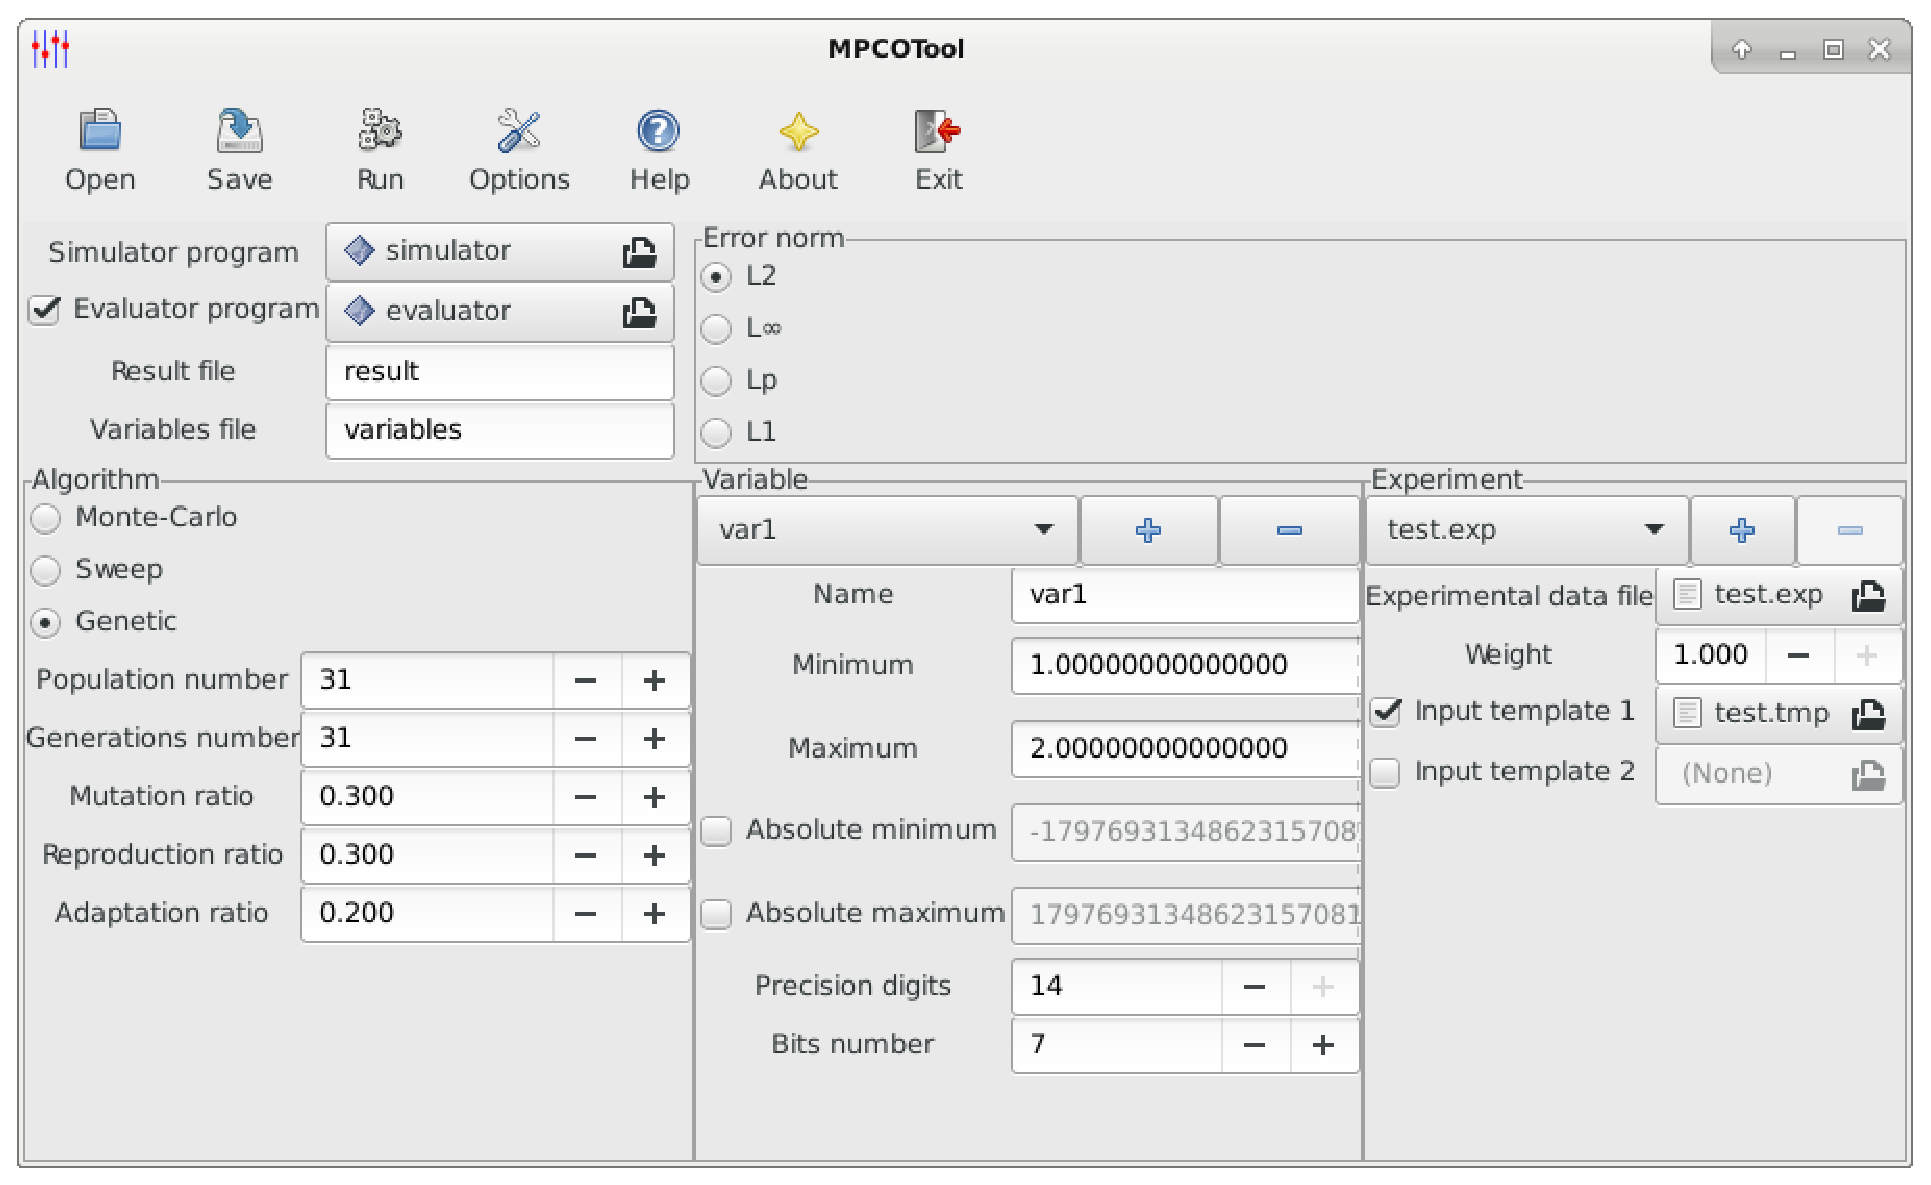
\includegraphics[width=9.30cm]{mpcotool-en.eps}
	\caption{Main window of MPCOTool graphical user interface application.
		\label{FigWindow}}
\end{figure}

Final optime results are presented in a dialog as the shown in the
figure~\ref{FigResult}.
\begin{figure}[ht!]
	\centering
	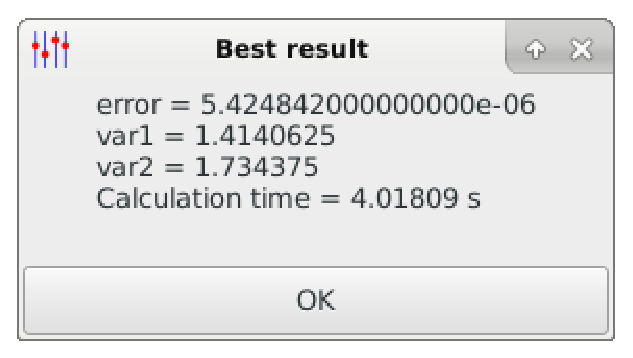
\includegraphics[width=2.87cm]{result-en.eps}
	\caption{Results dialog of MPCOTool graphical user interface application.
		\label{FigResult}}
\end{figure}

\section{Input files}

\subsection{Main input file}

\subsubsection{XML format}

This file can be written in XML format with a tree type structure as the
represented in figure~\ref{FigMainFile}.
\psset{xunit=0.4mm,yunit=0.4mm}
\PSPICTURE{0}{-115}{280}{25}
{
	\tiny
	\psframe(0,-5)(280,25)
	\psline(40,-5)(40,25)
	\rput(20,20){\bf optimize}
	\rput(60,20){\bf simulator}
	\rput(95,20){\bf algorithm}
	\rput(130,20){evaluator}
	\rput(165,20){nsimulations}
	\rput(205,20){niterations}
	\rput(240,20){tolerance}
	\rput(265,20){nbest}
	\rput(60,10){threshold}
	\rput(95,10){npopulation}
	\rput(135,10){ngenerations}
	\rput(170,10){mutation}
	\rput(205,10){reproduction}
	\rput(240,10){adaptation}
	\rput(265,10){seed}
	\rput(60,0){climbing}
	\rput(95,0){nsteps}
	\rput(130,0){nestimates}
	\rput(170,0){relaxation}
	\rput(200,0){norm}
	\rput(217,0){p}
	\rput(235,0){result}
	\rput(260,0){variables}
	\psline(20,-5)(20,-15)(40,-15)
	\psframe(40,-20)(280,-10)
	\psline(80,-20)(80,-10)
	\rput(60,-15){\bf experiment}
	\rput(95,-15){\bf name}
	\rput(125, -15){\bf template$_\mathbf{1}$}
	\rput(160,-15){template$_2$}
	\rput(195,-15){$\cdots$}
	\rput(230,-15){template$_n$}
	\rput(260,-15){weight}
	\psline(20,-15)(20,-25)
	\rput(140,-30){$\cdots$}
	\psline(20,-35)(20,-45)(40,-45)
	\psframe(40,-50)(280,-40)
	\psline(80,-50)(80,-40)
	\rput(60,-45){\bf experiment}
	\rput(95,-45){\bf name}
	\rput(125,-45){\bf template$_\mathbf{1}$}
	\rput(160,-45){template$_2$}
	\rput(195,-45){$\cdots$}
	\rput(230,-45){template$_n$}
	\rput(260,-45){weight}
	\psline(20,-45)(20,-65)(40,-65)
	\psframe(40,-75)(280,-55)
	\psline(80,-75)(80,-55)
	\rput(60,-60){\bf variable}
	\rput(95,-60){\bf name}
	\rput(120,-60){\bf minimum}
	\rput(152.5,-60){\bf maximum}
	\rput(195,-60){absolute\_minimum}
	\rput(250,-60){absolute\_maximum}
	\rput(100,-70){precision}
	\rput(130,-70){nsweeps}
	\rput(155,-70){nbits}
	\rput(175,-70){step}
	\psline(20,-65)(20,-80)
	\rput(140,-85){$\cdots$}
	\psline(20,-90)(20,-105)(40,-105)
	\psframe(40,-115)(280,-95)
	\psline(80,-115)(80,-95)
	\rput(60,-100){\bf variable}
	\rput(95,-100){\bf name}
	\rput(120,-100){\bf minimum}
	\rput(152.5,-100){\bf maximum}
	\rput(195,-100){absolute\_minimum}
	\rput(250,-100){absolute\_maximum}
	\rput(100,-110){precision}
	\rput(130,-110){nsweeps}
	\rput(155,-110){nbits}
	\rput(175,-110){step}
}{Structure of the main input file. Mandatory nodes and properties are in bold.
Others properties can be also mandatory depending on the selected optimization
algorithm}{FigMainFile}

The main XML node has to begin with the key label \emph{"optimize"}. The
available properties are:
\begin{description}
	\item[simulator]: to indicate the simulator program,
	\item[evaluator]: optional. It specifies the evaluator program if required,
	\item[algorithm]: to set the optimization algorithm. Three values are
		currently available:
	\begin{description}
		\item[sweep]: sweep brute force algorithm. It requires for each
			variable:
		\begin{description}
			\item[nsweeps]: number of sweeps to generate each variable in every
			experiment,
		\end{description}
		\item[Monte-Carlo]: Monte-Carlo brute force algorithm. It requires on 
			the main XML node:
			\begin{description}
				\item[nsimulations]: number of simulations to run for each 
					iteration in every experiment,
			\end{description}
		\item[genetic]: genetic algorithm. It requires the following parameters 
			in the main XML node:
			\begin{description}
				\item[npopulation]: number of population entities,
				\item[ngenerations]: number of generations,
				\item[mutation]: mutation ratio,
				\item[reproduction]: reproduction ratio,
				\item[adaptation]: adaptation ratio.
			\end{description}
			And for each variable:
			\begin{description}
				\item[nbits]: number of bits to encode each variable,
			\end{description}
		\item[orthogonal]: orthogonal sampling brute force algorithm. It 
			requires for each variable:
		\begin{description}
			\item[nsweeps]: number of sweeps to generate each variable in every
			experiment,
		\end{description}
	\end{description}
	\item[niterations]: number of iterations (default 1) to perform the
		iterative algorithm,
	\item[nbest]: number of best simulations to calculate convergence interval
		on next iteration for the iterative algorithm (default 1),
	\item[tolerance]: tolerance parameter to relax the convergence interval of
		the iterative algorithm (default 0),
	\item[threshold]: threshold in the objective function to stop the
		optimization,
	\item[seed]: seed of the pseudo-random numbers generator (default 7007),
	\item[climbing]: method to search the optimal climbing (optional for brute
		force algorithms). Two values are currently available:
	\begin{description}
		\item[coordinates]: coordinates climbing,
		\item[random]: random climbing. It requieres:
		\begin{description}
			\item[nestimates]: number of random checks to search the optimal
				climbing.
		\end{description}
	\end{description}
	Both methods requires the following parameters:
	\begin{description}
		\item[nsteps]: number of steps to perform the hill climbing method,
		\item[relaxation]: relaxation parameter for the hill climbing method,
	\end{description}
	and for each variable:
	\begin{description}
		\item[step]: initial step size for the hill climbing method,
	\end{description}
	\item[norm]: to set the error norm (default "euclidian"). Four values are
		currently available:
		\begin{description}
			\item[euclidian]: euclidian error norm $L_2$, see
				(\ref{EqObjectiveFunctionLII}),
			\item[maximum]: maximum error norm $L_\infty$, see
				(\ref{EqObjectiveFunctionLi}),
			\item[p]: P error norm $L_p$. It requires:
			\begin{description}
				\item[p]: exponent of the P error norm, see
					(\ref{EqObjectiveFunctionLp}),
			\end{description}
			\item[taxicab]: taxicab error norm $L_1$, see
				(\ref{EqObjectiveFunctionLI}),
		\end{description}
	\item[result]: to set the result file name. Optional, the default file name
		is \emph{"result"},
	\item[variables]: to set the variables file name. Optional, the default file
		name is \emph{"variables"}.
\end{description}

The first type of child XML nodes has to begin with the key label
\emph{"experiment"}. It details the experimental data and it contains the properties:
\begin{description}
	\item[name]: name of the input data file with experimental results to calibrate,
	\item[templateX]: $X$-th input data file template for the simulation program,
	\item[weight]: weight (default 1) to apply in the objective function, see (\ref{EqObjectiveFunctionLII}) to (\ref{EqObjectiveFunctionLI}).
\end{description}

The second type of child XML nodes has to begin with the key label
\emph{"variable"}. It specifies the variables data and it has the properties:
\begin{description}
	\item[name]: variable label. On the $X$-th variable, the program parse all input
file templates creating the input simulation files by replacing all
@variableX@ labels by this name.
\item[minimum, maximum]: variable extreme values. The program creates the input
simulation files by replacing all @valueX@ labels in the input file templates
by a value between these extreme values on the $X$-th variable, depending on the
optimization algorithm,
\item[absolute\_minimum, absolute\_maximum]: absolute variable extreme values.
On iterative methods, the tolerance can increase initial \emph{minimum} or
\emph{maximum} values in each iteration. These values are the allowed extreme values
compatible with the model parameter limits,
\item[precision]: number of decimal digits of precision. 0 apply for integer numbers.
\end{description}

%%%%%%%%%%%%%%%%%%%%%%
In this format the file is written as:
\begin{lstlisting}[language=xml,basicstyle=\scriptsize]
<?xml version="1.0"?>
<optimize simulator="simulator_name" evaluator="evaluator_name"
	algorithm="algorithm_type" nsimulations="simulations_number"
	niterations="iterations_number" tolerance="tolerance_value"
	nbest="best_number" npopulation="population_number"
	ngenerations="generations_number" mutation="mutation_ratio"
	reproduction="reproduction_ratio" adaptation="adaptation_ratio"
	climbing="hill_climbing_type" nsteps="steps_number"
	relaxation="relaxation_parameter" nestimates="estimates_number"
	threshold="threshold_parameter" norm="norm_type" p="p_parameter"
	seed="random_seed" result_file="result_file"
	variables_file="variables_file">
    <experiment name="data_file_1" template1="template_1_1"
		template2="template_1_2" ... weight="weight_1"/>
    ...
    <experiment name="data_file_N" template1="template_N_1"
		template2="template_N_2" ... weight="weight_N"/>
    <variable name="variable_1" minimum="min_value" maximum="max_value"
		precision="precision_digits" sweeps="sweeps_number"
		nbits="bits_number" step="step_size"/>
    ...
    <variable name="variable_M" minimum="min_value" maximum="max_value"
		precision="precision_digits" sweeps="sweeps_number"
		nbits="bits_number" step="step_size"/>
</optimize>
\end{lstlisting}

Alternatively, the main input file can be also written in JSON format:
\begin{lstlisting}[language=json,basicstyle=\scriptsize]
{
	"simulator": "simulator_name",
	"evaluator": "evaluator_name",
	"algorithm": "algorithm_type",
	"nsimulations": "simulations_number",
	"niterations": "iterations_number",
	"tolerance": "tolerance_value",
	"nbest": "best_number",
	"npopulation": "population_number",
	"ngenerations": "generations_number",
	"mutation": "mutation_ratio",
	"reproduction": "reproduction_ratio",
	"adaptation": "adaptation_ratio",
	"climbing": "hill_climbing_type",
	"nsteps": "steps_number",
	"relaxation": "relaxation_parameter",
	"nestimates": "estimates_number",
	"threshold": "threshold_parameter",
	"norm": "norm_type",
	"p": "p_parameter",
	"seed": "random_seed",
	"result_file": "result_file",
	"variables_file": "variables_file",
	"experiments":
	[
		{
			"name": "data_file_1",
			"template1": "template_1_1",
			"template2": "template_1_2",
			...
			"weight": "weight_1",
		},
	    ...
		{
			"name": "data_file_N",
			"template1": "template_N_1",
			"template2": "template_N_2",
			...
			"weight": "weight_N",
		}
	],
	"variables":
	[
		{

			"name": "variable_1",
			"minimum": "min_value",
			"maximum": "max_value",
			"precision": "precision_digits",
			"sweeps": "sweeps_number",
			"nbits": "bits_number",
			"step": "step_size",
		},
		...
		{
			"name": "variable_M",
			"minimum": "min_value",
			"maximum": "max_value",
			"precision": "precision_digits",
			"sweeps": "sweeps_number",
			"nbits": "bits_number",
			"step": "step_size",
		}
	]
}
\end{lstlisting}
%%%%%%%%%%%%%%%%%%%%%%

\subsection{Template files}

$N_{experiments}\times N_{inputs}$
template files must be written to reproduce every input file associated to every experiment (see figure~\ref{FigStructure}). All the template files are syntactically analyzed by MPCOTool to replace the labels as follows in order to generate the simulation program input files:
\begin{description}
\item[@variableX@]: is replaced by the label associated to the $X$-th empirical parameter defined in \emph{main input file};
\item[@valueX@]: is replaced by the value associated to the $X$-th empirical parameter calculated by the optimization algorithm using the data defined in \emph{main input file};
\end{description}

\section{Output files}

\subsection{Results file}

MPCOTool generates a file where the best combination of variables and the
corresponding calculated objective function, as well as the calculation time,
are saved. The file name can be set ih the \emph{result} property of the main
input file. If not set the default file name is "result".

\subsection{Variables file}

The program generates also a file where all combinations
of variables checked in the calibration are saved in columns. First columns
correspond to the variables combination and the last column is the objective
function value. The file name can be set in the \emph{varaibles} property of the
main input file. A default name "variables" is used if this property is not
defined.

\chapter{Organization of MPCOTool}

Let us assume that $N_{parameters}$ empirical parameters are sought desired so
that the results from a simulation model are the best fit to $N_{experiments}$
experimental data and that the simulator requires $N_{inputs}$ input files. The
structure followed by MPCOTool is summarized in the \emph{main input file},
where both $N_{experiments}$ and $N_{inputs}$ are specified. Furthermore, it
contains the extreme values of the empirical parameters and the chosen
optimization algorithm. Then, MPCOTool reads the corresponding
$N_{experiments}\times N_{inputs}$ templates to build the simulator input files
replacing key labels by empirical parameter values created by the optimization
algorithm. There are two options: either the simulator compares directly the
simulation results with the \emph{experimental data file}, hence generating a
file with the value of the error; or another external program, defined in the
property \emph{evaluator}, is invoked to compare with the \emph{experimental
data file} and to produce the error value. In both cases this error value is
saved in an \emph{objective value file}. Then for each experiment, an objective
value $o_i$ is obtained. The final value of the objective function ($J$)
associated with the experiments set can be calculated by four different error
norms:
\EQ{L_2:\quad J=\sqrt{\sum_{i=1}^{N_{experiments}}\ABS{w_i\,o_i}^2},}
{EqObjectiveFunctionLII}
\EQ{L_\infty:\quad J=\max_{i=1}^{N_{experiments}}\ABS{w_i\,o_i},}
{EqObjectiveFunctionLi}
\EQ{L_p:\quad J=\sqrt[p]{\sum_{i=1}^{N_{experiments}}\ABS{w_i\,o_i}^p},}
{EqObjectiveFunctionLp}
\EQ{L_1:\quad J=\sum_{i=1}^{N_{experiments}}\ABS{w_i\,o_i},}
{EqObjectiveFunctionLI}
with $w_i$ the weight associated to the $i$-th experiment, specified in the
\emph{main input file}. Figure~\ref{FigStructure} is a sketch of the
structure.
\psset{xunit=0.4mm,yunit=0.4mm}
\PSPICTURE{-25}{-115}{260}{55}
{
	\tiny
	\rput(10,50){Main input file}
	\psframe(-20,45)(40,55)
	\psline{->}(40,50)(50,50)
	\rput(10,25){1st template file}
	\psframe(-20,20)(40,30)
	\psline{->}(40,25)(50,25)
	\psline[linestyle=dotted,dotsep=1pt]{->}(50,25)(90,25)
	\rput(10,15){$\cdots$}
	\rput(10,5){$n$-th template file}
	\psframe(-20,0)(40,10)
	\psline{->}(40,5)(50,5)
	\psline[linestyle=dotted,dotsep=1pt]{->}(50,5)(90,5)
	\rput(10,-35){$\cdots$}
	\rput(10,-75){$(N\,n)$-th template file}
	\psframe(-20,-70)(40,-80)
	\psline{->}(40,-75)(50,-75)
	\psline[linestyle=dotted,dotsep=1pt]{->}(50,-75)(90,-75)
	\rput(70,50){MPCOTool}
	\psframe(50,-95)(90,55)
	\rput(70,-110){Objective function value}
	\psframe(35,-105)(105,-115)
	\psline{->}(70,-95)(70,-105)
	\psline{->}(90,25)(100,25)
	\psline{->}(90,5)(100,5)
	\psline{->}(90,-55)(100,-55)
	\psline{->}(90,-75)(100,-75)
	\rput(120,5){$n$-th input file}
	\psframe(100,0)(140,10)
	\psline{->}(140,5)(150,5)
	\rput(120,15){$\cdots$}
	\rput(120,25){1st input file}
	\psframe(100,20)(140,30)
	\psline{->}(140,25)(145,25)(145,5)
	\rput(175,5){Simulator}
	\psframe(150,0)(200,10)
	\psline[linestyle=dashed,dash=2pt 1pt]{->}(175,10)(175,20)
	\psline[linestyle=dashed,dash=2pt 1pt]{->}(200,5)(210,7.5)
	\rput(175,25){Results file}
	\psframe[linestyle=dashed,dash=3pt 1pt](150,20)(200,30)
	\psline[linestyle=dashed,dash=2pt 1pt]{->}(200,25)(210,30)
	\rput(175,45){Experimental}
	\rput(175,40){data file}
	\psframe(150,35)(200,50)
	\psline[linestyle=dashed,dash=2pt 1pt]{->}(200,42.5)(210,30)
	\psline[linestyle=dashed,dash=2pt 1pt]{->}(150,42.5)(145,42.5)(145,25)
	\rput(230,30){Evaluator}
	\psline[linestyle=dashed,dash=2pt 1pt]{->}(230,25)(230,15)
	\psframe[linestyle=dashed,dash=3pt 1pt](210,25)(250,35)
	\rput(230,10){Objective}
	\rput(230,5){value file}
	\psframe(210,0)(250,15)
	\psline{->}(250,7.5)(260,7.5)(260,-90)(90,-90)
	\psline[linestyle=dotted,dotsep=1pt]{->}(90,-90)(70,-90)(70,-95)
	\rput(120,50){1st experiment}
	\psframe[linestyle=dotted](95,-5)(255,55)
	\rput(175,-15){$\cdots$}
	\rput(120,-75){$n$-th input file}
	\psframe(100,-80)(140,-70)
	\psline{->}(140,-75)(150,-75)
	\rput(120,-65){$\cdots$}
	\rput(120,-55){1st input file}
	\psframe(100,-60)(140,-50)
	\psline{->}(140,-55)(145,-55)(145,-75)
	\rput(175,-75){Simulator}
	\psframe(150,-80)(200,-70)
	\psline[linestyle=dashed,dash=2pt 1pt]{->}(175,-70)(175,-60)
	\psline[linestyle=dashed,dash=2pt 1pt]{->}(200,-75)(210,-72.5)
	\rput(175,-55){Results file}
	\psframe[linestyle=dashed,dash=3pt 1pt](150,-60)(200,-50)
	\psline[linestyle=dashed,dash=2pt 1pt]{->}(200,-55)(210,-50)
	\rput(175,-35){Experimental}
	\rput(175,-40){data file}
	\psframe(150,-30)(200,-45)
	\psline[linestyle=dashed,dash=2pt 1pt]{->}(200,-37.5)(210,-50)
	\psline[linestyle=dashed,dash=2pt 1pt]{->}(150,-37.5)(145,-37.5)(145,-55)
	\rput(230,-50){Evaluator}
	\psline[linestyle=dashed,dash=2pt 1pt]{->}(230,-55)(230,-65)
	\psframe[linestyle=dashed,dash=3pt 1pt](210,-55)(250,-45)
	\rput(230,-70){Objective}
	\rput(230,-75){value file}
	\psframe(210,-80)(250,-65)
	\psline(250,-72.5)(260,-72.5)
	\rput(120,-30){$N$-th experiment}
	\psframe[linestyle=dotted](95,-85)(255,-25)
}{Flowchart of the interactions among MPCOTool, the input files and the
simulation and evaluation programs to produce an objective function value for
each empirical parameters combination generated by the optimization algorithm}
{FigStructure}

The whole process is repeated for each combination of empirical parameters generated by the optimization algorithm. Furthermore, MPCOTool automatically parallelizes the simulations using all the available computing resources.

\chapter{Optimization methods}

The optimization methods implemented in MPCOTool are next presented. The following notation will be used:
\begin{description}
	\item[$N_{simulations}$]: number of simulations made for each iteration,
	\item[$N_{iterations}$]: number of iterations on iterative methods,
	\item[$N_{total}$]: total number of simulations.
\end{description}
In iterative methods $N_{total}=N_{simulations}\times N_{iterations}$.
In pure brute force methods
$N_{iterations}=1\;\Rightarrow\;N_{total}=N_{simulations}$.

\section{Sweep brute force method}

The sweep brute force method finds the optimal set of parameters within a solution region by dividing it into regular subdomains. To find the optimal solution, the domain interval $x_i \in \PA{x_{i,min},\,x_{i,max}}$ is first defined for each variable $x_i$. Then, a regular partition in  $N_{x,i}$ subintervals is made. Taking into account this division of the solution space, the number of required simulations is:
\EQ{N_{simulations}=N_{x,1}\times N_{x,2}\times\cdots,}
{EqNSweeps}
where $N_{x,i}$ is the number of sweeps in the variable $x_i$.

In figure~\ref{FigSweep} the $(x,y)$ domain is defined by the intervals $x\in\PA{x_{min},\,x_{max}}$ and $y \in \PA{y_{min},\,y_{max}}$. Both $x$ and $y$ intervals are divided into 5 regions with $N_{x}=N_{y}=5$. The optimal will be found within the region by evaluating the error of each $\PA{x_i,\,y_i}$ set of parameters hence requiring 25 evaluations. Note that the computational cost increases strongly as the number of variables grow.

\PICTURE{210}{200}
{
	\put(20,10){\vector(0,1){180}}
	\put(20,10){\vector(1,0){180}}
	\put(10,190){$y$}
	\put(200,0){$x$}
	\multiput(50,40)(30,0){5}{\qbezier[40](0,0)(0,60)(0,120)}
	\multiput(50,40)(0,30){5}{\qbezier[40](0,0)(60,0)(120,0)}
	\multiput(50,40)(30,0){5}{\multiput(0,0)(0,30){5}{\circle*{2}}}
	\qbezier[10](50,10)(50,25)(50,40)
	\put(40,0){$x_{\min}$}
	\qbezier[10](170,10)(170,25)(170,40)
	\put(160,0){$x_{\max}$}
	\qbezier[10](20,40)(35,40)(50,40)
	\put(0,37){$y_{\min}$}
	\qbezier[10](20,160)(35,160)(50,160)
	\put(0,157){$y_{\max}$}
}{Diagram showing an example of application of the sweep brute force method
with two variables for $N_x=N_y=5$}{FigSweep}

Brute force algorithms present low convergence rates but they are strongly
parallelizable because every simulation is completely independent. If the
computer, or the computers cluster, can execute $N_{tasks}$ parallel tasks
every task do $N_{total}/N_{tasks}$ simulations, obviously taking into account
rounding effects (every task has to perform a natural number of simulations).
In figure~\ref{FigBruteForceParallelization} a flowchart of this parallelization
scheme is represented. Being independent each task, a distribution on different
execution threads may be performed exploding the full parallel capabilities of
the machine where MPCOTool is run.

\psset{xunit=0.5mm,yunit=0.5mm}
\PSPICTURE{-90}{-55}{90}{-15}
{
	\tiny
	\rput(0,-15){Generation of $N_{total}$ empirical parameters sets}
	\psframe(-55,-20)(55,-10)
	\psline{->}(0,-20)(-50,-25)
	\psline{->}(0,-20)(0,-25)
	\psline{->}(0,-20)(55,-25)
	\rput(-55,-30){1st task:}
	\rput(-55,-35){$N_{total}/N_{tasks}$ simulations}
	\psframe(-90,-25)(-20,-40)
	\rput(0,-32.5){$\cdots$}
	\rput(55,-30){$N_{tasks}$-th task:}
	\rput(55,-35){$N_{total}/N_{tasks}$ simulations}
	\psframe(20,-25)(90,-40)
	\psline{->}(-55,-40)(0,-45)
	\psline{->}(0,-40)(0,-45)
	\psline{->}(55,-40)(0,-45)
	\rput(0,-50){Getting optimal empirical parameters set}
	\psframe(-50,-45)(50,-55)
}{Flowchart of the parallelization scheme in MPCOTool for brute force methods
(sweep and Monte-Carlo)}{FigBruteForceParallelization}

\section{Monte-Carlo method}

Monte-Carlo based methods run simulations using aleatory values of the
variables assuming  uniform probability within the extreme values range.
Figure~\ref{FigMonteCarlo} shows the structure of an example using two
variables.

\PICTURE{210}{200}
{
	\put(20,10){\vector(0,1){180}}
	\put(20,10){\vector(1,0){180}}
	\put(10,190){$y$}
	\put(200,0){$x$}
	\put(69,159){\circle*{2}}
	\put(163,73){\circle*{2}}
	\put(108,67){\circle*{2}}
	\put(139,154){\circle*{2}}
	\put(138,104){\circle*{2}}
	\put(129,131){\circle*{2}}
	\put(146,77){\circle*{2}}
	\put(70,102){\circle*{2}}
	\put(97,97){\circle*{2}}
	\put(75,66){\circle*{2}}
	\put(90,43){\circle*{2}}
	\put(163,63){\circle*{2}}
	\put(157,109){\circle*{2}}
	\put(109,119){\circle*{2}}
	\put(71,107){\circle*{2}}
	\put(64,75){\circle*{2}}
	\put(127,47){\circle*{2}}
	\put(126,127){\circle*{2}}
	\put(61,125){\circle*{2}}
	\put(62,123){\circle*{2}}
	\put(110,55){\circle*{2}}
	\put(84,64){\circle*{2}}
	\put(65,49){\circle*{2}}
	\put(59,105){\circle*{2}}
	\put(156,75){\circle*{2}}	
	\qbezier[50](50,10)(50,85)(50,160)
	\put(40,0){$x_{\min}$}
	\qbezier[50](170,10)(170,85)(170,160)
	\put(160,0){$x_{\max}$}
	\qbezier[50](20,40)(95,40)(170,40)
	\put(0,37){$y_{\min}$}
	\qbezier[50](20,160)(95,160)(170,160)
	\put(0,157){$y_{\max}$}
}{Diagram illustrating a Monte-Carlo brute force method with two variables and
$N_{simulations}=25$}{FigMonteCarlo}

Monte-Carlo method is also easily parallelizable following a strategy as the
flowchart represented in the figure~\ref{FigBruteForceParallelization}.

\section{Iterative algorithm applied to brute force methods}

MPCOTool allows to iterate both sweep or Monte-Carlo brute force methods in
order to seek convergence. In this case, the best results from the previous
iteration are used to force new intervals in the variables for the following
iteration. Then for $N_{best}^j$, the subset of the best simulation results in
the $j$-th iteration, the following quantities are defined:
\begin{description}
\item[$\displaystyle x_{\max}^b=\max_{i\in N_{best}}x_i^j$]: Maximum value of
	variable $x$ in the subset of the best simulation results from the $j$-th
	iteration.
\item[$\displaystyle x_{\min}^b=\max_{i\in N_{best}}x_i^j$]: Minimum value of
	variable $x$ in the subset of the best simulation results from the $j$-th
	iteration.
\end{description}
A new interval in the variable $x$ is defined to build the optimization values in the next $(j+1)$-th iteration so that:
\EQ{x_i^{j+1}\in\left[x_{\min}^{j+1},\;x_{\max}^{j+1}\right],}
{EqIterationInterval}
with:
\[
	\mathrm{Sweep}\;\Rightarrow\;\left\{\begin{array}{c}
	\displaystyle
	x_{\max}^{j+1}=x_{\max}^b+\frac{x_{\max}^j-x_{\min}^j}{N_x-1}\,tolerance,\\
	\displaystyle
	x_{\min}^{j+1}=x_{\min}^b-\frac{x_{\min}^j-x_{\min}^j}{N_x-1}\,tolerance,\\
	\end{array}\right.
\]
\EQ
{
	\mathrm{Monte-Carlo}\;\Rightarrow\;\left\{\begin{array}{c}
	\displaystyle x_{\max}^{j+1}=\frac{x_{\max}^b+x_{\min}^b
	+\left(x_{\max}^b-x_{\min}^b\right)(1+tolerance)}{2},\\
	\displaystyle x_{\min}^{j+1}=\frac{x_{\max}^b+x_{\min}^b
	-\left(x_{\max}^b-x_{\min}^b\right)(1+tolerance)}{2},
	\end{array}\right.
}{EqIterationIntervalII}
being $tolerance$ a factor increasing the size of the variable intervals to
simulate the next iteration.
Figure~\ref{FigIterative} contains a sketch of the procedure used by the the iterative algorithm to modify the variables intervals in order to enforce convergence. 

\PICTURE{210}{400}
{
	\small
	\multiput(0,0)(0,200){2}
	{
		\put(20,10){\vector(0,1){180}}
		\put(20,10){\vector(1,0){180}}
		\put(10,190){$y$}
		\put(200,0){$x$}
	}
	\put(90,380){1st iteration}
	\put(50,370){*: best results}
	\put(69,359){\circle*{2}}
	\put(163,273){\circle*{2}}
	\put(108,267){*}
	\put(139,354){\circle*{2}}
	\put(138,304){*}
	\put(129,331){\circle*{2}}
	\put(146,277){\circle*{2}}
	\put(70,302){\circle*{2}}
	\put(97,297){*}
	\put(75,266){\circle*{2}}
	\put(90,243){\circle*{2}}
	\put(163,263){\circle*{2}}
	\put(157,309){\circle*{2}}
	\put(109,319){*}
	\put(71,307){\circle*{2}}
	\put(64,275){\circle*{2}}
	\put(127,247){\circle*{2}}
	\put(126,327){\circle*{2}}
	\put(61,325){\circle*{2}}
	\put(62,323){\circle*{2}}
	\put(110,255){\circle*{2}}
	\put(84,264){\circle*{2}}
	\put(65,249){\circle*{2}}
	\put(59,305){\circle*{2}}
	\put(156,275){\circle*{2}}	
	\qbezier[50](50,210)(50,285)(50,360)
	\put(40,200){$x_{\min}^1$}
	\qbezier[50](170,210)(170,285)(170,360)
	\put(160,200){$x_{\max}^1$}
	\qbezier[50](20,240)(95,240)(170,240)
	\put(0,237){$y_{\min}^1$}
	\qbezier[50](20,360)(95,360)(170,360)
	\put(0,357){$y_{\max}^1$}
	\qbezier[21](99,272)(119.5,272)(140,272)
	\qbezier[21](99,324)(119.5,324)(140,324)
	\qbezier[26](99,272)(99,298)(99,324)
	\qbezier[26](140,272)(140,298)(140,324)
	\put(99,267){\vector(1,0){41}}
	\put(140,267){\vector(-1,0){41}}
	\put(95,255){$x_{\max}^b-x_{\min}^b$}
	\put(94.9,215){\vector(1,0){49.2}}
	\put(144.1,215){\vector(-1,0){49.2}}
	\put(95,220){$x_{\max}^2-x_{\min}^2$}
	\qbezier[20](99,272)(96.95,241)(94.9,210)
	\qbezier[20](140,272)(142.05,241)(144.1,210)
	\qbezier[26](99,272)(69.5,269.4)(20,266.8)
	\qbezier[26](99,324)(69.5,326.6)(20,329.2)
	\put(80,180){2nd iteration}
	\put(102,123){\circle*{2}}
	\put(141,83){\circle*{2}}
	\put(118,80){\circle*{2}}
	\put(131,121){\circle*{2}}
	\put(131,97){\circle*{2}}
	\put(127,110){\circle*{2}}
	\put(134,84){\circle*{2}}
	\put(103,96){\circle*{2}}
	\put(114,94){\circle*{2}}
	\put(105,79){\circle*{2}}
	\put(111,68){\circle*{2}}
	\put(141,78){\circle*{2}}
	\put(139,100){\circle*{2}}
	\put(119,104){\circle*{2}}
	\put(103,98){\circle*{2}}
	\put(100,83){\circle*{2}}
	\put(126,70){\circle*{2}}
	\put(126,108){\circle*{2}}
	\put(99,107){\circle*{2}}
	\put(100,106){\circle*{2}}
	\put(119,74){\circle*{2}}
	\put(109,78){\circle*{2}}
	\put(101,71){\circle*{2}}
	\put(99,98){\circle*{2}}
	\put(138,83){\circle*{2}}
	\qbezier[40](94.9,10)(94.9,69.6)(94.9,129.2)
	\put(84.9,0){$x_{\min}^2$}
	\qbezier[40](144.1,10)(144.1,69.6)(144.1,129.2)
	\put(134.1,0){$x_{\max}^2$}
	\qbezier[41](20,129.2)(82.05,129.2)(144.1,129.2)
	\put(0,126.2){$y_{\max}^2$}
	\qbezier[41](20,66.8)(82.05,66.8)(144.1,66.8)
	\put(0,63.8){$y_{\min}^2$}
}{Diagram representing an example of the iterative algorithm applied to a
Monte-Carlo brute force method with two variables for $N_{simulations}= 25$,
$N_{best}=4$ and two iterations}{FigIterative}

The iterative algorithm can be also easily parallelized. However, this method is
less parallelizable than pure brute force methods because the parallelization
has to be performed for each iteration (see a flowchart in the
figure~\ref{FigIterativeParallelization}).

\psset{xunit=0.5mm,yunit=0.5mm}
\PSPICTURE{-100}{-130}{100}{-15}
{
	\tiny
	\rput(0,-15){1st iteration:}
	\rput(0,-20){Generation of $N_{simulations}$ empirical parameters sets}
	\psframe(-60,-25)(60,-10)
	\psline{->}(0,-25)(-60,-30)
	\psline{->}(0,-25)(0,-30)
	\psline{->}(0,-25)(60,-30)
	\rput(-60,-35){1st task:}
	\rput(-60,-40){$N_{simulations}/N_{tasks}$ simulations}
	\psframe(-100,-30)(-20,-45)
	\rput(0,-37.5){$\cdots$}
	\rput(60,-35){$N_{tasks}$-th task:}
	\rput(60,-40){$N_{simulations}/N_{tasks}$ simulations}
	\psframe(20,-30)(100,-45)
	\psline{->}(-60,-45)(0,-50)
	\psline{->}(0,-45)(0,-50)
	\psline{->}(60,-45)(0,-50)
	\rput(0,-55){Getting $N_{best}$ empirical parameters sets}
	\psframe(-55,-50)(55,-60)
	\psline{->}(0,-60)(0,-65)
	\rput(0,-70){$\cdots$}
	\psline{->}(0,-75)(0,-80)
	\rput(0,-85){$N_{iterations}$-th iteration:}
	\rput(0,-90){Generation of $N_{simulations}$ empirical parameters sets}
	\psframe(-60,-95)(60,-80)
	\psline{->}(0,-95)(-60,-100)
	\psline{->}(0,-95)(0,-100)
	\psline{->}(0,-95)(60,-100)
	\rput(-60,-105){1st task:}
	\rput(-60,-110){$N_{simulations}/N_{tasks}$ simulations}
	\psframe(-100,-100)(-20,-115)
	\rput(0,-107.5){$\cdots$}
	\rput(60,-105){$N_{tasks}$-th task:}
	\rput(60,-110){$N_{simulations}/N_{tasks}$ simulations}
	\psframe(20,-100)(100,-115)
	\psline{->}(-60,-115)(0,-120)
	\psline{->}(0,-115)(0,-120)
	\psline{->}(60,-115)(0,-120)
	\rput(0,-125){Getting optimal empirical parameters set}
	\psframe(-55,-120)(55,-130)
}{Flowchart of the parallelization scheme in MPCOTool for the iterative
method}{FigIterativeParallelization}

\section{Direction search method}

Brute force optimization methods, sweep and Monte-Carlo, can be also combined
with a direction search algorithm. Defining the vector $\vec{r}_i$ as the optime
variables combination obtained in the $i$-th step, $\vec{r}_1$ as the optime
varaibles combination vector obtained by the brute force method and defining
the vector $\vec{s}_i$ as:
\EQ
{
	\vec{s}_1=\vec{0},\qquad
	\vec{s}_i=(1-relaxation)\,\vec{s}_{i-1}+relaxation\,\Delta\vec{r}_{i-1},
}{Eqs}
with $\Delta\vec{r}_{i-1}=\vec{r}_i+\vec{r}_{i-1}$ and $relaxation$ the
relaxation parameter, the direction search method checks $N_{estimates}$
variable combinations and choice the optimum as:
\EQ
{
	\vec{r}_{i+1}=\mathrm{optime}\PA{\vec{r}_i,\;\vec{r}_i+\vec{s}_i+\vec{t}_j},
	\;j=1,\cdots,N_{estimates}.
}{EqDirection}
If the step does not improve the optimum ($\vec{r}_i=\vec{r}_{i+1}$) then the
direction step vectors $\vec{t}_j$ are divided by two and $\vec{s}_{i+1}$ is set
to zero. The method is iterated $N_{steps}$ times.

Although direction search method gets the fastest convergence, is the method in
MPCOTool that obtains the least advantages of parallelization. The method is
almost sequential and parallelization only can be performed for each step in
the $N_{estimates}$ simulations to estimate the optimal direction. In the
figure~\ref{FigDirectionParallelization} a flowchart of the parallelization
scheme for this method is shown.

\psset{xunit=0.5mm,yunit=0.5mm}
\PSPICTURE{-100}{-130}{100}{-15}
{
	\tiny
	\rput(0,-15){1st step:}
	\rput(0,-20){Generation of $N_{estimates}$ empirical parameters sets}
	\psframe(-60,-25)(60,-10)
	\psline{->}(0,-25)(-60,-30)
	\psline{->}(0,-25)(0,-30)
	\psline{->}(0,-25)(60,-30)
	\rput(-60,-35){1st task:}
	\rput(-60,-40){$N_{estimates}/N_{tasks}$ simulations}
	\psframe(-100,-30)(-20,-45)
	\rput(0,-37.5){$\cdots$}
	\rput(60,-35){$N_{tasks}$-th task:}
	\rput(60,-40){$N_{estimates}/N_{tasks}$ simulations}
	\psframe(20,-30)(100,-45)
	\psline{->}(-60,-45)(0,-50)
	\psline{->}(0,-45)(0,-50)
	\psline{->}(60,-45)(0,-50)
	\rput(0,-55){Getting optimal empirical parameters set}
	\psframe(-55,-50)(55,-60)
	\psline{->}(0,-60)(0,-65)
	\rput(0,-70){$\cdots$}
	\psline{->}(0,-75)(0,-80)
	\rput(0,-85){$N_{steps}$-th step:}
	\rput(0,-90){Generation of $N_{estimates}$ empirical parameters sets}
	\psframe(-60,-95)(60,-80)
	\psline{->}(0,-95)(-60,-100)
	\psline{->}(0,-95)(0,-100)
	\psline{->}(0,-95)(60,-100)
	\rput(-60,-105){1st task:}
	\rput(-60,-110){$N_{estimates}/N_{tasks}$ simulations}
	\psframe(-100,-100)(-20,-115)
	\rput(0,-107.5){$\cdots$}
	\rput(60,-105){$N_{tasks}$-th task:}
	\rput(60,-110){$N_{estimates}/N_{tasks}$ simulations}
	\psframe(20,-100)(100,-115)
	\psline{->}(-60,-115)(0,-120)
	\psline{->}(0,-115)(0,-120)
	\psline{->}(60,-115)(0,-120)
	\rput(0,-125){Getting optimal empirical parameters set}
	\psframe(-55,-120)(55,-130)
}{Flowchart of the parallelization scheme in MPCOTool for the direction search
method}{FigDirectionParallelization}

MPCOTool uses two methods to build the $\vec{t}_j$ vectors:

\subsection{Coordinates descent}

This method builds the $\vec{t}_j$ vectors by increasing or decreasing only one
variable:
\[
	\vec{t}_1=\MATRIX{c}{step_1\\0\\0\\\vdots\\0},\quad
	\vec{t}_2=\MATRIX{c}{-step_1\\0\\0\\\vdots\\0},\quad
	\vec{t}_3=\MATRIX{c}{0\\step_2\\0\\\vdots\\0},
\]
\EQ
{
	\vec{t}_4=\MATRIX{c}{0\\-step_2\\0\\\vdots\\0},\quad\cdots\quad,
	\vec{t}_{N_{estimates}}=\MATRIX{c}{0\\0\\0\\\vdots\\
	-step_{N_{variables}}},
}{EqtDescent}
being $step_j$ the initial step size for the $j$-th variable defined by the user
in the main input file. The number of estimates in this method depends on the
variables number:
\EQ{N_{estimates}=2\,N_{variables}}{EqNestimatesDescent}

\subsection{Random}

The vectors $\vec{t}_j$ are built randomly as:
\EQ
{
	\vec{t}_j=\MATRIX{c}{\PA{1-2\,r_{j,1}}\,step_1\\\vdots\\
	\PA{1-2\,r_{j,k}}\,step_k\\\vdots\\
	\PA{1-2\,r_{j,N_{variables}}}\,step_{N_{variables}}},
}{EqtRandom}
with $r_{j,k}\in[0,1)$ random numbers.

In the figure~\ref{FigDirection} a sketch for a system with two variables is
presented to illustrate the working mode of coordinates descent and random
algorithms.
\psset{xunit=0.45mm,yunit=0.45mm,runit=0.5mm}
\PSPICTURE{0}{0}{260}{100}
{
	\psline{->}(10,10)(10,90)
	\rput(15,95){$variable_2$}
	\psline{->}(10,10)(120,10)
	\rput(110,5){$variable_1$}
	\rput(20,15){$\vec{r}_{i-1}$}
	\pscircle*(20,20){1}
	\rput(55,34){$\vec{r}_i$}
	\pscircle*(55,40){1}
	\psline{->}(20,20)(55,40)
	\rput(30,36){$\Delta\vec{r}_{i-1}$}
	\psline{->}(55,40)(90,65)
	\rput(65,54){$\vec{s}_i$}
	\psline{->}(90,65)(90,85)
	\pscircle*(90,85){1}
	\rput(95,81){$\vec{t}_3$}
	\psline{->}(90,65)(110,65)
	\pscircle*(110,65){1}
	\rput(105,71){$\vec{t}_1$}
	\psline{->}(90,65)(70,65)
	\pscircle*(70,65){1}
	\rput(75,70){$\vec{t}_2$}
	\psline{->}(90,65)(90,45)
	\pscircle*(90,45){1}
	\rput(95,50){$\vec{t}_4$}
	\psline{->}(140,10)(140,90)
	\rput(145,95){$variable_2$}
	\psline{->}(140,10)(250,10)
	\rput(240,5){$variable_1$}
	\rput(150,15){$\vec{r}_{i-1}$}
	\pscircle*(150,20){1}
	\rput(185,34){$\vec{r}_i$}
	\pscircle*(185,40){1}
	\psline{->}(150,20)(185,40)
	\rput(160,36){$\Delta\vec{r}_{i-1}$}
	\psline{->}(185,40)(220,65)
	\rput(195,54){$\vec{s}_i$}
	\psline{->}(220,65)(207,75)
	\pscircle*(207,75){1}
	\rput(207,81){$\vec{t}_3$}
	\psline{->}(220,65)(228,68)
	\pscircle*(228,68){1}
	\rput(228,74){$\vec{t}_1$}
	\psline{->}(220,65)(212,49)
	\pscircle*(212,49){1}
	\rput(212,43){$\vec{t}_2$}
}{(Left) coordinates descent and (right) random with $N_{estimates}=3$ direction
search method checks of variables combination in a system with two variables}
{FigDirection}

\section{Genetic method}

MPCOTool also offers the use of a genetic method \cite{genetic} with its default algorithms.
It is inspired on the ideas in \citet{gaul}, but it has been fully reprogrammed involving more modern external libraries.
The code in Genetic is also open source under BSD license. Figure~\ref{FigGeneticFlow} shows the flowchart of the genetic method implemented in Genetic.

\psset{xunit=0.5mm,yunit=0.5mm}
\PSPICTURE{-120}{-185}{120}{20}
{
	\tiny
	\rput(0,15){Generation of $N_{population}$}
	\rput(0,10){random genomes}
	\psframe(-35,5)(35,20)
	\psline{->}(0,5)(0,0)
	\rput(0,-5){$generation=1$}
	\psframe(-25,-10)(25,0)
	\psline{->}(0,-10)(0,-15)
	\rput(0,-20){Simulation of the $N_{population}$}
	\rput(0,-25){entities}
	\psframe(-40,-30)(40,-15)
	\psline{->}(0,-30)(0,-35)
	\rput(0,-40){Sorting the $N_{population}$}
	\rput(0,-45){entities by objective function value}
	\psframe(-45,-50)(45,-35)
	\psline{->}(0,-50)(0,-55)
	\rput(0,-60){Eliminating the worst}
	\rput(0,-65){$N_{mutation}+N_{reproduction}+N_{adaptation}$ entities}
	\psframe(-65,-70)(65,-55)
	\psline{->}(0,-70)(-80,-75)
	\rput(-80,-80){Generation of $N_{mutation}$}
	\rput(-80,-85){new entities by mutation}
	\psframe(-115,-90)(-45,-75)
	\psline{->}(-80,-90)(-80,-95)
	\rput(-80,-100){Simulation of the $N_{mutation}$}
	\rput(-80,-105){new mutated entities}
	\psframe(-115,-110)(-45,-95)
	\psline{->}(0,-70)(0,-75)
	\rput(0,-80){Generation of $N_{reproduction}$}
	\rput(0,-85){new entities by reproduction}
	\psframe(-40,-90)(40,-75)
	\psline{->}(0,-90)(0,-95)
	\rput(0,-100){Simulation of the $N_{reproduction}$}
	\rput(0,-105){new reproduced entities}
	\psframe(-40,-110)(40,-95)
	\psline{->}(0,-70)(82.5,-75)
	\rput(82.5,-80){Generation of $N_{adaptation}$}
	\rput(82.5,-85){new entities by adaptation}
	\psframe(120,-90)(45,-75)
	\psline{->}(82.5,-90)(82.5,-95)
	\rput(82.5,-100){Simulation of the $N_{adaptation}$}
	\rput(82.5,-105){new adapted entities}
	\psframe(120,-110)(45,-95)
	\psline{->}(-80,-110)(0,-115)
	\psline{->}(0,-110)(0,-115)
	\psline{->}(82.5,-110)(0,-115)
	\rput(0,-120){Sorting the old $N_{survival}$ entities and the new}
	\rput(0,-125){$N_{mutation}+N_{reproduction}+N_{adaptation}$ entities}
	\rput(0,-130){by objective function values}
	\psframe(-65,-115)(65,-135)
	\psline{->}(0,-135)(0,-140)
	\rput(0,-145){Increase $+1$ $generation$}
	\psframe(-30,-140)(30,-150)
	\psline{->}(0,-150)(0,-155)
	\rput(0,-162.5){$generation<N_{generations}$?}
	\pspolygon(-50,-162.5)(0,-170)(50,-162.5)(0,-155)
	\psline{->}(-50,-162.5)(-120,-162.5)(-120,-62.5)(-65,-62.5)
	\rput(-60,-160){Yes}
	\rput(-5,-172.5){No}
	\psline{->}(0,-170)(0,-175)
	\rput(0,-180){Select the best entity}
	\psframe(-30,-185)(30,-175)
}{Flow diagram of the genetic method implemented in Genetic}{FigGeneticFlow}

\subsection{The genome}

The variables to calibrate/optimize are coded in Genetic using a bit chain: the
genome. The larger the number of bits assigned to a variable the higher the resolution.
The number of bits assigned to each variable, and therefore the genome size, is fixed and the same for all the 
simulations. Figure~\ref{FigGenome} shows an example for the coding of three variables. The value assigned to a variable $x$ is determined by the allowed extreme values $x_{\min}$ and $x_{\max}$, the binary number assigned in the genome to variable $I_x$ and by the number of bits assigned to variable $N_x$ according to
the following formula:
\EQ{x=x_{\min}+\frac{I_x}{2^{N_x}-1}\,\left(x_{\max}-x_{\min}\right).}{EqGenome}

\psset{unit=1mm}
\PSPICTURE{0}{0}{80}{30}
{
	\scriptsize
	\rput(40,27){Genome}
	\rput(15,23){Variable 1}
	\pspolygon(0,15)(30,15)(30,20)(0,20)
	\rput(40,23){Variable 2}
	\pspolygon(30,15)(50,15)(50,20)(30,20)
	\rput(65,23){Variable 3}
	\pspolygon(50,15)(80,15)(80,20)(50,20)
	\psline{->}(10,12)(0,12)
	\rput(5,9){Less}
	\rput(5,6){significant}
	\rput(5,3){bit}
	\psline{->}(20,12)(30,12)
	\rput(25,9){More}
	\rput(25,6){significant}
	\rput(25,3){bit}
	\rput(2,17.5){1}
	\rput(4,17.5){0}
	\rput(6,17.5){0}
	\rput(8,17.5){1}
	\rput(10,17.5){0}
	\rput(12,17.5){0}
	\rput(14,17.5){1}
	\rput(16,17.5){1}
	\rput(18,17.5){1}
	\rput(20,17.5){1}
	\rput(22,17.5){1}
	\rput(24,17.5){1}
	\rput(26,17.5){0}
	\rput(28,17.5){1}
	\rput(32,17.5){1}
	\rput(34,17.5){0}
	\rput(36,17.5){0}
	\rput(38,17.5){0}
	\rput(40,17.5){0}
	\rput(42,17.5){0}
	\rput(44,17.5){0}
	\rput(46,17.5){0}
	\rput(48,17.5){0}
	\rput(52,17.5){1}
	\rput(54,17.5){1}
	\rput(56,17.5){1}
	\rput(58,17.5){1}
	\rput(60,17.5){0}
	\rput(62,17.5){1}
	\rput(64,17.5){0}
	\rput(66,17.5){0}
	\rput(68,17.5){0}
	\rput(70,17.5){0}
	\rput(72,17.5){1}
	\rput(74,17.5){1}
	\rput(76,17.5){1}
	\rput(78,17.5){1}
}{Example coding three variables to optimize into a
genome. The first and third variables have been coded with 14 bits, and the second
variable has been coded with 9 bits}{FigGenome}

\subsection{Survival of the best individuals}

In a population with $N_{population}$ individuals, in the first generation all the cases are simulated. The input variables are
taken from the genome of each individual. Next, in every generation, $N_{population}\times R_{mutation}$ individuals are generated by mutation, $N_{population}\times R_{reproduction}$ individuals are generated by reproduction and $N_{population}\times R_{adaptation}$ individuals are generated by adaptation, obviously
taking into account rounding. On second and further generations only simulations
associated to this new individuals ($N_{new}$) have to be run:
\EQ
{
	N_{new}=N_{population}
	\times\left(R_{mutation}+R_{reproduction}+R_{adaptation}\right).
}{EqNew}
Then, total number of simulations performed by the genetic algorithm is:
\EQ
{
	N_{total}=N_{population}+\left(N_{generations}-1\right)\times N_{new},
}{EqGeneticNumber}
with $N_{generations}$ the number of generations of new entities.
The individuals of the former population that obtained lower values in the evaluation function are replaced so that the best $N_{survival}$ individuals survive:
\EQ
{
	N_{survival}=N_{population}-N_{new}.
}{EqSurvival}
Furthermore, the ancestors to generate new individuals are chosen among the surviving population. Obviously, to have survival population, the following condition has to be enforced:
\EQ{R_{mutation}+R_{reproduction}+R_{adaptation}<1}{EqSurvivalCondition}
MPCOTool uses a default aleatory criterion in Genetic, with a probability linearly decreasing with the ordinal in the ordered set of surviving individuals (see figure~\ref{FigSelection}).

\PICTURE{250}{110}
{
	\scriptsize
	\put(10,20){\vector(0,1){80}}
	\put(10,20){\vector(1,0){235}}
	\put(0,102){Probability to be selected as parent}
	\put(30,0){Survival population sorted by objective function values}
	\multiput(20,20)(10,0){2}{\line(0,1){66}}
	\put(20,86){\line(1,0){10}}
	\put(19,10){1st}
	\multiput(40,20)(10,0){2}{\line(0,1){60}}
	\put(40,80){\line(1,0){10}}
	\put(39,10){2nd}
	\multiput(60,20)(10,0){2}{\line(0,1){54}}
	\put(60,74){\line(1,0){10}}
	\put(59,10){3rd}
	\multiput(80,20)(10,0){2}{\line(0,1){48}}
	\put(80,68){\line(1,0){10}}
	\put(79,10){4th}
	\multiput(100,20)(10,0){2}{\line(0,1){42}}
	\put(100,62){\line(1,0){10}}
	\put(140,10){...}
	\multiput(120,20)(10,0){2}{\line(0,1){36}}
	\put(120,56){\line(1,0){10}}
	\multiput(140,20)(10,0){2}{\line(0,1){30}}
	\put(140,50){\line(1,0){10}}
	\multiput(160,20)(10,0){2}{\line(0,1){24}}
	\put(160,44){\line(1,0){10}}
	\multiput(180,20)(10,0){2}{\line(0,1){18}}
	\put(180,38){\line(1,0){10}}
	\multiput(200,20)(10,0){2}{\line(0,1){12}}
	\put(200,32){\line(1,0){10}}
	\multiput(220,20)(10,0){2}{\line(0,1){6}}
	\put(220,26){\line(1,0){10}}
	\put(205,10){$N_{survival}$-th}
	\qbezier[54](10,90.5)(127.5,50.25)(245,20)
}{Probability of a survival entity to be selected as parent
of the new entities generated by mutation, reproduction or adaptation
algorithms}{FigSelection}

\subsection{Mutation algorithm}

In the mutation algorithm an identical copy of the parent genome is made except for a bit, randomly chosen with uniform probability, which is inverted. Figure~\ref{FigMutation} shows an example of the procedure.
\psset{unit=1mm}
\PSPICTURE{0}{0}{80}{20}
{
	\scriptsize
	\rput(10,17.5){Parent}
	\pspolygon(20,15)(80,15)(80,20)(20,20)
	\rput(22,17.5){1}
	\rput(24,17.5){1}
	\rput(26,17.5){0}
	\rput(28,17.5){1}
	\rput(30,17.5){1}
	\rput(32,17.5){1}
	\rput(34,17.5){0}
	\rput(36,17.5){0}
	\rput(38,17.5){0}
	\rput(40,17.5){0}
	\rput(42,17.5){0}
	\rput(44,17.5){0}
	\rput(46,17.5){0}
	\rput(48,17.5){0}
	\rput(50,17.5){1}
	\rput(52,17.5){1}
	\rput(54,17.5){1}
	\rput(56,17.5){1}
	\rput(58,17.5){1}
	\rput(60,17.5){0}
	\rput(62,17.5){1}
	\rput(64,17.5){0}
	\rput(66,17.5){0}
	\rput(68,17.5){0}
	\rput(70,17.5){0}
	\rput(72,17.5){1}
	\rput(74,17.5){1}
	\rput(76,17.5){1}
	\rput(78,17.5){1}
	\rput(10,2.5){Son}
	\pspolygon(20,0)(80,0)(80,5)(20,5)
	\rput(22,2.5){1}
	\rput(24,2.5){1}
	\rput(26,2.5){0}
	\rput(28,2.5){1}
	\rput(30,2.5){1}
	\rput(32,2.5){1}
	\rput(34,2.5){0}
	\rput(36,2.5){1}
	\rput(38,2.5){0}
	\rput(40,2.5){0}
	\rput(42,2.5){0}
	\rput(44,2.5){0}
	\rput(46,2.5){0}
	\rput(48,2.5){0}
	\rput(50,2.5){1}
	\rput(52,2.5){1}
	\rput(54,2.5){1}
	\rput(56,2.5){1}
	\rput(58,2.5){1}
	\rput(60,2.5){0}
	\rput(62,2.5){1}
	\rput(64,2.5){0}
	\rput(66,2.5){0}
	\rput(68,2.5){0}
	\rput(70,2.5){0}
	\rput(72,2.5){1}
	\rput(74,2.5){1}
	\rput(76,2.5){1}
	\rput(78,2.5){1}
	\psline{->}(50,15)(50,5)
	\rput(60,10){Mutation}
	\pspolygon(35,15)(37,15)(37,20)(35,20)
	\pspolygon(35,5)(37,5)(37,0)(35,0)
	\psline{->}(32,10)(36,10)(36,15)
	\psline{->}(32,10)(36,10)(36,5)
	\rput(16,10){Inversion of a random bit}
}{Diagram showing an example of the generation of a new entity by mutation}
{FigMutation}

\subsection{Reproduction algorithm}

The default algorithm in Genetic selects two different parents with one of the least errors after the 
complete simulation of one generation. 
A new individual is then generated by sharing the common bits of both parents and a random choice in the others.
The new child has the same number of bits as the parents and different genome. Figure~\ref{FigReproduction} shows a sketch
of the algorithm.

\psset{unit=1mm}
\PSPICTURE{0}{0}{80}{20}
{
	\scriptsize
	\multido{\rb=0+7.5,\rt=5+7.5}{3}
	{
		\psframe[linecolor=gray,fillcolor=gray,fillstyle=solid](20,\rb)(23,\rt)
		\psframe[linecolor=gray,fillcolor=gray,fillstyle=solid](25,\rb)(29,\rt)
		\psframe[linecolor=gray,fillcolor=gray,fillstyle=solid](45,\rb)(47,\rt)
		\psframe[linecolor=gray,fillcolor=gray,fillstyle=solid](49,\rb)(51,\rt)
		\psframe[linecolor=gray,fillcolor=gray,fillstyle=solid](59,\rb)(61,\rt)
		\psframe[linecolor=gray,fillcolor=gray,fillstyle=solid](63,\rb)(67,\rt)
		\psframe[linecolor=gray,fillcolor=gray,fillstyle=solid](71,\rb)(75,\rt)
	}
	\rput(10,17.5){1st parent}
	\psframe(20,15)(80,20)
	\rput(22,17.5){1}
	\rput(24,17.5){1}
	\rput(26,17.5){0}
	\rput(28,17.5){1}
	\rput(30,17.5){1}
	\rput(32,17.5){1}
	\rput(34,17.5){0}
	\rput(36,17.5){0}
	\rput(38,17.5){0}
	\rput(40,17.5){0}
	\rput(42,17.5){0}
	\rput(44,17.5){0}
	\rput(46,17.5){0}
	\rput(48,17.5){0}
	\rput(50,17.5){1}
	\rput(52,17.5){1}
	\rput(54,17.5){1}
	\rput(56,17.5){1}
	\rput(58,17.5){1}
	\rput(60,17.5){0}
	\rput(62,17.5){1}
	\rput(64,17.5){0}
	\rput(66,17.5){0}
	\rput(68,17.5){0}
	\rput(70,17.5){0}
	\rput(72,17.5){1}
	\rput(74,17.5){1}
	\rput(76,17.5){1}
	\rput(78,17.5){1}
	\rput(10,2.5){2nd parent}
	\psframe(20,0)(80,5)
	\rput(22,2.5){1}
	\rput(24,2.5){0}
	\rput(26,2.5){0}
	\rput(28,2.5){1}
	\rput(30,2.5){0}
	\rput(32,2.5){0}
	\rput(34,2.5){1}
	\rput(36,2.5){1}
	\rput(38,2.5){1}
	\rput(40,2.5){1}
	\rput(42,2.5){1}
	\rput(44,2.5){1}
	\rput(46,2.5){0}
	\rput(48,2.5){1}
	\rput(50,2.5){1}
	\rput(52,2.5){0}
	\rput(54,2.5){0}
	\rput(56,2.5){0}
	\rput(58,2.5){0}
	\rput(60,2.5){0}
	\rput(62,2.5){0}
	\rput(64,2.5){0}
	\rput(66,2.5){0}
	\rput(68,2.5){1}
	\rput(70,2.5){1}
	\rput(72,2.5){1}
	\rput(74,2.5){1}
	\rput(76,2.5){0}
	\rput(78,2.5){0}
	\rput(10,10){Son}
	\psframe(20,7.5)(80,12.5)
	\rput(22,10){1}
	\rput(24,10){0}
	\rput(26,10){0}
	\rput(28,10){1}
	\rput(30,10){0}
	\rput(32,10){0}
	\rput(34,10){0}
	\rput(36,10){1}
	\rput(38,10){1}
	\rput(40,10){0}
	\rput(42,10){1}
	\rput(44,10){1}
	\rput(46,10){0}
	\rput(48,10){1}
	\rput(50,10){1}
	\rput(52,10){1}
	\rput(54,10){1}
	\rput(56,10){1}
	\rput(58,10){0}
	\rput(60,10){0}
	\rput(62,10){0}
	\rput(64,10){0}
	\rput(66,10){0}
	\rput(68,10){1}
	\rput(70,10){0}
	\rput(72,10){1}
	\rput(74,10){1}
	\rput(76,10){0}
	\rput(78,10){1}
	\psline{->}(50,5)(50,7.5)
	\psline{->}(50,15)(50,12.5)
	\psline{->}(10,5)(10,7.5)
	\psline{->}(10,15)(10,12.5)
}{Example of the generation of a new entity by
reproduction in the Genetic default algorithm. Note that the identical bits in both parents (in grey) are also present in their son. The rest of the bits are random}{FigReproduction}

\subsection{Adaptation algorithm}

Another algorithm is included in Genetic called "adaptation" although, in the
biological sense, it would be rather be a smooth mutation. First, one of the
variables codified in the genome is randomly selected with uniform probability.
Then, a bit is randomly chosen assuming a probability linearly decreasing with
the significance of the bit. The new individual receives a copy of the parents
genome with the selected bit inverted. Figure~\ref{FigAdaptation} contains an
example.

\psset{unit=1mm}
\PSPICTURE{-30}{-7.5}{80}{30}
{
	\scriptsize
	\rput(-10,17.5){Parent}
	\rput(15,23){Variable 1}
	\psframe(0,15)(30,20)
	\rput(40,23){Variable 2}
	\psframe(30,15)(50,20)
	\rput(65,23){Variable 3}
	\psline{->}(55,28)(65,28)(65,26)
	\rput(35,28){Random selection of a variable}
	\psframe(55,21)(75,26)
	\psframe(50,15)(80,20)
	\psline{->}(10,12)(0,12)
	\rput(5,9){Less}
	\rput(5,6){significant}
	\rput(5,3){bit}
	\psline{->}(20,12)(30,12)
	\rput(25,9){More}
	\rput(25,6){significant}
	\rput(25,3){bit}
	\rput(2,17.5){1}
	\rput(4,17.5){0}
	\rput(6,17.5){0}
	\rput(8,17.5){1}
	\rput(10,17.5){0}
	\rput(12,17.5){0}
	\rput(14,17.5){1}
	\rput(16,17.5){1}
	\rput(18,17.5){1}
	\rput(20,17.5){1}
	\rput(22,17.5){1}
	\rput(24,17.5){1}
	\rput(26,17.5){0}
	\rput(28,17.5){1}
	\rput(32,17.5){1}
	\rput(34,17.5){0}
	\rput(36,17.5){0}
	\rput(38,17.5){0}
	\rput(40,17.5){0}
	\rput(42,17.5){0}
	\rput(44,17.5){0}
	\rput(46,17.5){0}
	\rput(48,17.5){0}
	\rput(52,17.5){1}
	\rput(54,17.5){1}
	\rput(56,17.5){1}
	\rput(58,17.5){1}
	\rput(60,17.5){0}
	\rput(62,17.5){1}
	\rput(64,17.5){0}
	\rput(66,17.5){0}
	\rput(68,17.5){0}
	\rput(70,17.5){0}
	\rput(72,17.5){1}
	\rput(74,17.5){1}
	\rput(76,17.5){1}
	\rput(78,17.5){1}
	\rput(65,10){Probability of selection}
	\rput(65,7){of a bit}
	\psframe[fillcolor=gray,fillstyle=solid](77,0)(79,0.5)
	\psframe[fillcolor=gray,fillstyle=solid](75,0)(77,1.0)
	\psframe[fillcolor=gray,fillstyle=solid](73,0)(75,1.5)
	\psframe[fillcolor=gray,fillstyle=solid](71,0)(73,2.0)
	\psframe[fillcolor=gray,fillstyle=solid](69,0)(71,2.5)
	\psframe[fillcolor=gray,fillstyle=solid](67,0)(69,3.0)
	\psframe[fillcolor=gray,fillstyle=solid](65,0)(67,3.5)
	\psframe[fillcolor=gray,fillstyle=solid](63,0)(65,4.0)
	\psframe[fillcolor=gray,fillstyle=solid](61,0)(63,4.5)
	\psframe[fillcolor=gray,fillstyle=solid](59,0)(61,5.0)
	\psframe[fillcolor=gray,fillstyle=solid](57,0)(59,5.5)
	\psframe[fillcolor=gray,fillstyle=solid](55,0)(57,6.0)
	\psframe[fillcolor=gray,fillstyle=solid](53,0)(55,6.5)
	\psframe[fillcolor=gray,fillstyle=solid](51,0)(53,7.0)
	\rput(-10,-5){Son}
	\psframe(0,-2.5)(30,-7.5)
	\psframe(30,-2.5)(50,-7.5)
	\psframe(50,-2.5)(80,-7.5)
	\rput(2,-5){1}
	\rput(4,-5){0}
	\rput(6,-5){0}
	\rput(8,-5){1}
	\rput(10,-5){0}
	\rput(12,-5){0}
	\rput(14,-5){1}
	\rput(16,-5){1}
	\rput(18,-5){1}
	\rput(20,-5){1}
	\rput(22,-5){1}
	\rput(24,-5){1}
	\rput(26,-5){0}
	\rput(28,-5){1}
	\rput(32,-5){1}
	\rput(34,-5){0}
	\rput(36,-5){0}
	\rput(38,-5){0}
	\rput(40,-5){0}
	\rput(42,-5){0}
	\rput(44,-5){0}
	\rput(46,-5){0}
	\rput(48,-5){0}
	\rput(52,-5){1}
	\rput(54,-5){1}
	\rput(56,-5){0}
	\rput(58,-5){1}
	\rput(60,-5){0}
	\rput(62,-5){1}
	\rput(64,-5){0}
	\rput(66,-5){0}
	\rput(68,-5){0}
	\rput(70,-5){0}
	\rput(72,-5){1}
	\rput(74,-5){1}
	\rput(76,-5){1}
	\rput(78,-5){1}
	\psline{->}(-10,15)(-10,-2.5)
	\rput(-20,6.25){Adaptation}
	\psframe(55,-7.5)(57,-2.5)
	\psframe(55,15)(57,20)
}{Example of the generation of a new individual from a parent by adaptation}
{FigAdaptation}

This algorithm is rather similar to the mutation algorithm previously described but, since the probability to affect bits less significant is larger, so is the probability to produce smaller changes.

\subsection{Parallelization}

This method is also easily parallelizable following a similar scheme to the
iterative algorithm, as it can be seen in the
figure~\ref{FigGeneticParallelization}.

\psset{xunit=0.5mm,yunit=0.5mm}
\PSPICTURE{-100}{-185}{100}{-15}
{
	\tiny
	\rput(0,-15){1st generation:}
	\rput(0,-20){Generation of $N_{population}$ empirical parameters sets}
	\psframe(-60,-25)(60,-10)
	\psline{->}(0,-25)(-60,-30)
	\psline{->}(0,-25)(0,-30)
	\psline{->}(0,-25)(60,-30)
	\rput(-60,-35){1st task:}
	\rput(-60,-40){$N_{population}/N_{tasks}$ simulations}
	\psframe(-100,-30)(-20,-45)
	\rput(0,-37.5){$\cdots$}
	\rput(60,-35){$N_{tasks}$-th task:}
	\rput(60,-40){$N_{population}/N_{tasks}$ simulations}
	\psframe(20,-30)(100,-45)
	\psline{->}(-60,-45)(0,-50)
	\psline{->}(0,-45)(0,-50)
	\psline{->}(60,-45)(0,-50)
	\rput(0,-55){Getting $N_{survival}$ empirical parameters sets}
	\psframe(-55,-50)(55,-60)
	\psline{->}(0,-60)(0,-65)
	\rput(0,-70){2nd generation:}
	\rput(0,-75){Generation of $N_{new}$ empirical parameters sets}
	\psframe(-55,-80)(55,-65)
	\psline{->}(0,-80)(-60,-85)
	\psline{->}(0,-80)(0,-85)
	\psline{->}(0,-80)(60,-85)
	\rput(-55,-90){1st task:}
	\rput(-55,-95){$N_{new}/N_{tasks}$ simulations}
	\psframe(-90,-85)(-20,-100)
	\rput(0,-92.5){$\cdots$}
	\rput(55,-90){$N_{tasks}$-th task:}
	\rput(55,-95){$N_{new}/N_{tasks}$ simulations}
	\psframe(20,-85)(90,-100)
	\psline{->}(-55,-100)(0,-105)
	\psline{->}(0,-100)(0,-105)
	\psline{->}(55,-100)(0,-105)
	\rput(0,-110){Getting $N_{survival}$ empirical parameters sets}
	\psframe(-55,-105)(55,-115)
	\psline{->}(0,-115)(0,-120)
	\rput(0,-125){$\cdots$}
	\psline{->}(0,-130)(0,-135)
	\rput(0,-140){$N_{generations}$-th generation:}
	\rput(0,-145){Generation of $N_{new}$ empirical parameters sets}
	\psframe(-55,-150)(55,-135)
	\psline{->}(0,-150)(-60,-155)
	\psline{->}(0,-150)(0,-155)
	\psline{->}(0,-150)(60,-155)
	\rput(-55,-160){1st task:}
	\rput(-55,-165){$N_{new}/N_{tasks}$ simulations}
	\psframe(-90,-155)(-20,-170)
	\rput(0,-162.5){$\cdots$}
	\rput(55,-160){$N_{tasks}$-th task:}
	\rput(55,-165){$N_{new}/N_{tasks}$ simulations}
	\psframe(20,-155)(90,-170)
	\psline{->}(-55,-170)(0,-175)
	\psline{->}(0,-170)(0,-175)
	\psline{->}(55,-170)(0,-175)
	\rput(0,-180){Getting optimal empirical parameters set}
	\psframe(-55,-175)(55,-185)
}{Flowchart of the parallelization scheme implemented in Genetic for the genetic
method}{FigGeneticParallelization}

\clearpage
\renewcommand{\bibname}{References}
\addcontentsline{toc}{chapter}{\bibname}
\bibliography{bib}

\end{document}
